% Chapter Template

\chapter{Literature Review} % Main chapter title

\label{Chapter2} % Change X to a consecutive number; for referencing this chapter elsewhere, use \ref{ChapterX}

This chapter provides background information on the reasoning behind the secure phone project.
This consists of; (\ref{chap2sec1}) an introduction into the state of complex modern processors, (\ref{chap2sec2}) a brief history of computer processors, (\ref{chap2sec3}) a study into the verification of CPUs, which includes a graph detailing the large rise in the number of transistors per employee per new processor released, (\ref{chap2sec4}) security vulnerabilities, which looks at cases where vulnerabilities have been found or are imminent, (\ref{chap2sec5}) a brief overview of One Time Pad, (\ref{chap2sec6}) secure phones, which looks at the history of past secure devices and technologies, (\ref{chap2sec7}) a brief overview of the MEGA65 project, (\ref{chap2sec8}) a description of the design software used for the project.

%----------------------------------------------------------------------------------------
%	SECTION 1
%----------------------------------------------------------------------------------------

\section{Literature Review}
\label{chap2sec1}

Since the beginning of modern pipelined microprocessors, computers have become increasingly complex.
This complexity can bring about vulnerabilities deep within the software and hardware of a computer.
Vulnerabilities are often found through dedicated research and analysis of the specific operating system or component, with the solution to the problem often taking a significant amount of time to find.
In some cases, it isn’t certain that a solution can be found without drastically altering the computer hardware or software. 
Smartphones have grown exponentially in terms of their development and their capabilities over the past decade.
This growth has led to a more complex processing unit and interface, which in turn, has brought about similar security concerns to ones that can be found within a computer \cite{RN27}.
The Apple A11 chip for example, used in the iPhone X, has a staggering four billion transistors \cite{RN28}, which is comparable to many high-end processors currently being released.
With the emphasis of smartphones being on functionality, and with brands using increased functionality as a major selling point, the security of these devices has suffered.
More functionality brings with it increased complexity, which leads to increased attack surfaces, culminating in increased volumes of vulnerabilities, as already seen in modern computers.
This literature review explores this space, summarising a brief history of CPUs, how CPUs are verified, security concerns, and previous research into secure phones as a prerequisite to considering how smartphones with radically improved security properties can be created.

%----------------------------------------------------------------------------------------
%	SECTION 2
%----------------------------------------------------------------------------------------

\section{A Brief History of Computer Processors}
\label{chap2sec2}

To begin delving into the complexity of modern processors, a look back into the history of computer processors can provide reasoning for the secure smartphone project. 
In 1968, the Intel Corporation was founded by Robert Noyce and Gordon Moore \cite{RN2}.
Eight years prior to this, IBM became the first company to automatically mass-produce transistors \cite{RN2}, with Moore becoming the namesake of Moore’s Law.
By 1971 the first microprocessor was introduced, the Intel 4004.
The Intel 4004 microprocessor was produced on two-inch wafers, compared to twelve-inch wafers used in present microprocessors, consisted of 2,300 transistors, and was unique in being the smallest microprocessor design that ever went into production \cite{RN5}.

\begin{figure}
	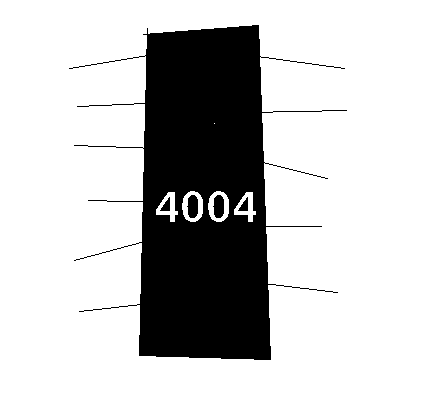
\includegraphics[width=\linewidth]{4004.jpg}
	\caption{Intel 4004 processor \cite{RN9}}
	\label{fig:4004}
\end{figure}

MOS Technology released the 6502 processor in 1975, with it consisting of 3,510 transistors.
At the time, the processor sold for less than one-sixth of the price of competing processors from larger companies \cite{RN29}.
The 6502 or its variations were used in popular home video game consoles such as the Atari 2600, Apple II, Nintendo Entertainment System and the Commodore 64.
Commodore International purchased MOS Technology outright soon after the 6502’s release \cite{RN29}.
The Intel 8080, consisting of 4,500 transistors, was released in April of 1974 and was a significant improvement over the Intel 4004 \cite{RN8}.
The 8-bit parallel central processing unit (CPU) was fabricated on a single LSI (Large Scale Integration) chip and used Intel’s n-channel silicon gate MOD process \cite{RN10}.
The successors to the 8080, in particular the 8086 – released in 1976 and the 8088 – released in 1979, were fundamental in the development of the modern, complex CPU.
The 8086 and 8088 incorporated a significant increase in transistors over their predecessor with each containing 29,000.
Many computers today still contain fundamental aspects of the 8086 chip \cite{RN11}.  
When the Motorola 68000 was released in 1980 it was one of the most powerful chips on the market \cite{RN18}.
With 68,000 transistors the chip was predominately used in the Apple Macintosh, Sun UNIX work stations, the Commodore Amiga line of computers, printers and video game consoles \cite{RN18}. 
In early 1993 Intel introduced the Pentium processor.
With 3.1 million transistors  \cite{RN13, Intel4584:online} the processor was the first to incorporate Intel’s super-scalar design.
Intel made large sacrifices of performance, power consumption and cost for the sake of maintaining the compatibility with legacy x86 code \cite{RN13}.
Intel estimated that 30\% of the Pentium’s transistors were used solely for providing x86 legacy support \cite{RN7}.
For this reason the processor lagged behind it’s RISC competitors in performance, while being more complex in its design.
In June of 1998 the Pentium II Xeon 400 processor was released, with it being the first Xeon processor.
The processor was the first Intel processor to be packaged in a cartridge, hosting a PCB with the CPU core as well as two or four L2 cache chips \cite{RN12} and consisted of 7.5 million transistors \cite{RN19}.
Intel’s plan was to have the Xeon provide a workstation performance at a lower price, while being able to run x86 workstation software on the same system as the normal office software \cite{RN12}.
Much later on in 2006 Intel released the Core 2 Duo processor, a significant improvement over the Pentium processors.
The processors started out with over 200 million transistors. 
This led to the start of the Core i3, i5 and i7 processors with the first generation being released in 2008 with the 8th generation being current.
The first i7 processors in 2008 started out having around 731 million transistors and as of today there as processors eclipsing 5 billion.  

As computers have become both faster and more powerful in all levels of execution they have consequently become far more complex and problematic to debug.
The latest Intel processor errata documents are longer than the entire operation manuals for their first processors ever made. The errata of modern processors is more complex than the entire definition of early CPUs \cite{6thGener70:online, mos6500m32:online}.

%----------------------------------------------------------------------------------------
%	SECTION 3
%----------------------------------------------------------------------------------------

\section{Verification of CPUs / Formal Analysis}
\label{chap2sec3}

One of the major issues manufacturers of modern computers face is functional verification.
In 2001 ARM released that their method of verifying their CPUs, so that the highest possible verification coverage could be achieved, was a process called ‘deterministic simulation’ \cite{RN6}.
This was a common and well understood methodology where test cases would be created to be used as self-checking assembler sequences.
These cases would then be re-run on a simulation test bench consisting of an ARM CPU, a simple memory model and some simple memory-mapped peripherals.
The tests would then be classified into two categories.
Although these tests singled out most errors within the CPU, full coverage of the system was not possible with this methodology.

Figure \ref{fig:transistor_graph} shows the number of transistors in a CPU divided by the number of employees at Intel against the processors of the given year.
Transistor count is a proxy for the complexity of a chip design, and employee count is a proxy for the amount of design verification effort that the company is able to apply.
That is, the graph approximates the complexity to verification effort ratio at Intel over several decades.
Higher values are worse, corresponding to reduced scrutiny of the design on a per-transistor basis.
While this measure is imperfect in a number of ways, including that Intel’s verification workforce may vary as a fraction of total work-force, and that it is expected that significant productivity increases are likely over the time period, for example through the creation of improved automated verification tools, it is obvious that this measure has increased by around five orders of magnitude over the 45 or so years covered.
While the data are not inclusive of every model of processor produced by Intel, it does also show a simultaneous trend to release more processors per unit time, thus spending the verification effort more thinly, even allowing that many contemporary models of processor will have large parts in common.

Circumstantial evidence of the difficulty of verifying modern complex processor designs, and that verification effort is being increasingly thinly spread, comes from the recent discovery of the Meltdown and Spectre attacks.
These attacks affect processors first produced a decade or more ago, as shown in Figure \ref{fig:transistor_graph}.
In the intervening time Intel, AMD and other makers of affected processors have produced many successive generations of processors, apparently without discovering these vulnerabilities.
The alternative hypothesis is that they did in fact know about it, and concealed this information.
If this were the case, then it would represent a very concerning situation, and would be an even stronger argument for the need for independently verifiable processor designs.
Many of the problems found within the hardware can require a full re-design of the processor to eliminate.

\begin{figure}
	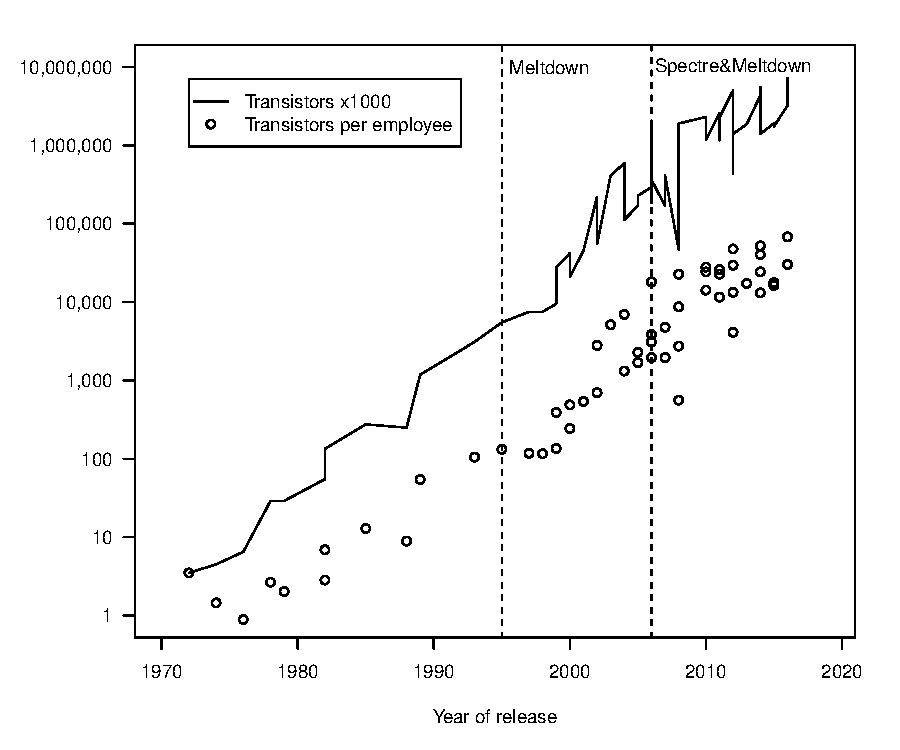
\includegraphics[width=\linewidth]{cpu-complexity/cpucomplexity.pdf}
	\caption{Transistors per number of employees at Intel against the number of transistors in their processors that year \cite{RN22, RN23, RN24, RN25, RN26}}
	\label{fig:transistor_graph}
\end{figure}

%----------------------------------------------------------------------------------------
%	SECTION 4
%----------------------------------------------------------------------------------------

\section{Security Vulnerabilities}
\label{chap2sec4}

In parallel with the rise of the number of transistors in a CPU there has also been a rise in the number of vulnerabilities and areas in which the CPU can be manipulated.
The number of reported software and hardware vulnerabilities grows constantly, with an approximate doubling rate beginning in 2017 \cite{RN17}.
The Spectre and Meltdown attacks (as previously mentioned) affect both the hardware and software of nearly every CPU from the past twenty years \cite{RN15}.
Spectre attacks involve causing a victim processor to speculatively perform operations that would not occur during correct program execution.
This can lead to the victim’s personal and confidential information being leaked via a side channel to the adversary \cite{RN16}.
Meltdown attacks predominately involve the hardware of a CPU, in particular the speculative execution features that allow a processor to reduce the time cost of branch instructions, by guessing whether the branch will be taken, and rolling back only if the guess was incorrect.
In particular, they rely on the fact that roll-back is not perfect, and that changes to cache occupancy changes can be detected post mortem, that can be used to deduce the contents of arbitrary memory locations to which the program has no permission to access \cite{RN3}.


%-----------------------------------
%	SUBSECTION 1
%-----------------------------------

\subsection{National Security Risks}

Effectively the same high-level security concern was raised in March of this year concerning the 5G network.
The Australian Government are aware that Huawei, a respected smartphone manufacturer in China, are intending to bring their 5G technology to Australia, which could potentially introduce new threats and vulnerabilities.
After having already been blocked from tendering for the National Broadband Network in 2012, 5G could potentially be an alternative to the NBN as well, which could potentially persuade customer’s preferences due to it having a faster mobile network.

The government’s concern is that Huawei’s technology could lead to security concerns down the track if there is a war between countries and Australia suddenly becomes a hostile adversary.
If Huawei were able to go ahead with their plan, eventually all mobile devices will be connected to the 5G network.
This would leave all 5G mobiles vulnerable to potential attacks, with the trust of security being left in the phone provider’s and network carrier’s hands.
The problem is not that any vulnerability in Huawei equipment has been identified, or even that there has been any proven intention to miss-use the technology in this way.
Rather, the problem is simply that the government is unable to be sure that this is not the case, and that uncertainty stems directly from the impossibility of fully verifying he hardware and software components of such complex systems.
Therefore, the government has had to assume that the possibility is a real risk to national society.
However, if the user was able to manually turn off the phone’s connection to this network, the threat of a potential attack would be mitigated \cite{RN14}.

%----------------------------------------------------------------------------------------
%	SECTION 5
%----------------------------------------------------------------------------------------

\section{One Time Pad}
\label{chap2sec5}

        The most secure solutions rely on One Time Pad (OTP) encryption, because this is the simplest scheme that offers unconditional security \cite{shannon-otp}.
        Unconditional security means that it does not matter how much effort an adversary may commit to breaking the security of the system, that they cannot succeed.
        That is, if an OTP scheme is correctly applied, it is not possible for an adversary to deduce the contents of communications enciphered with it.
        This is because each binary digit (or its equivalent, in analog systems) is enciphered using a separate key, which is never re-used.
        It therefore follows, that if any of these one-bit keys are correctly guessed, that they provide no information about any of the other keys. Put another way, it is impossible to determine if a guess for the value of a particular key is correct.
        Unconditionally secure systems like OTP are secure even in the face of Quantum Computing \cite{kabanov2018practical}.
        
%----------------------------------------------------------------------------------------
%	SECTION 6
%----------------------------------------------------------------------------------------

\section{Secure Telephony}
\label{chap2sec6}

	In the past there have been many attempts to create secure telephony devices, with varying success \cite{RN30}.
        Of interest to us, is SIGSALY, the first example of what was widely considered an unbreakable telephony system.
        
	SIGSALY was developed in 1941 as a digital speech encryption system.
        The limited technology of the time meant that each unit consisted of dozens of full-height racks of equipment.
        However, in operation, it was very similar to modern encrypted telephony:
        The voice to be transmitted was digitised to produce a very low bit rate data stream, which was then combined using modular arithmetical with cryptographic keys to produce the encrypted output. The process was reversed at the receiving end \cite{bennett1983secret,RN21}.

        The key material for SIGSALY was in the form of specially manufactured pairs of records, similar to normal music records of the era, where each digit of information was a tone representing a value between 0 and 5 \cite{bennett1983secret}.  The synchronisation required for the mechanical turn-tables was an engineering feat in itself.
        
        The records themselves were produced and distributed under extremely tight controls, because as with all OTP systems, the pad material must not be intercepted by an adversary, or else the entire system will be broken.
        Similarly, pad material must not be re-used, as otherwise it is possible to make inferences about the key material, as occurred in the Verona Project, when it was realised that some OTP material had been re-used by the soviets during the second world war\cite{cohen1997venona,mcgrew2002counter}.

        The SIGSALY system never suffered from the re-use of key material, as each record was carefully destroyed immediately after use,
        and it was used heavily in the latter period of World War II for confidential conversations between British Prime Minister Winston Churchill and United States President Franklin Roosevelt \cite{RN21}.
        The high cost of producing the records, each of which provided only twelve minutes of key material, the complications of safely transporting them to the remote ''telephones'', and the sheer size, power consumption and cost of the system meant that SIGSALY was only used for a period of four years, and only 12 SIGSALY systems were built\cite{RN21}.
    
\begin{figure}
	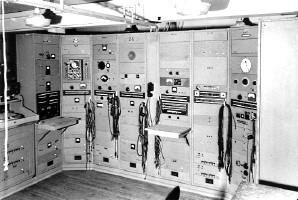
\includegraphics[width=\linewidth]{terminal.jpg}
	\caption{The transmitting side of a SIGSALY terminal \cite{RN21}}
	\label{fig:SIGSALY}
\end{figure}

The STU-I phone, a secure desk telephone used by the Government of the United States of America and its contractors, arrived in 1970.
It had a successor, the STU-II, and replaced the STU-I in 1975.
The third iteration, the STU-III was introduced in 1977, with it being on the first applications of asymmetric cryptography \cite{RN30}.
Today the United States Government still use STU phones for secure government telecommunications \cite{RN30}.

In terms of mobile phones, Blackberry sell themselves on producing secure phones.
When booted up, their smartphone’s system check both the hardware and software components on the device to ensure that nothing has been tampered with.
Full-disk encryption is also offered on the phones to protect private information as well as the choice for a numeric, alphanumeric or picture password.
The devices however are still based around a modern complex CPU and hence still have underlying vulnerabilities, for example in 2017 where Blackberry had to notify it’s users about the impact of “BlueBorne” \cite{RN20}, a collection of issues with the implementation of Bluetooth on a variety of software platforms. 
	It can be seen from the past that as the CPU in smartphones becomes more complex the ability to be able to secure it effectively decreases. 

%----------------------------------------------------------------------------------------
%	SECTION 7
%----------------------------------------------------------------------------------------

\section{MEGA 65 Project}
\label{chap2sec7}

The MEGA 65 Project is a joint venture of the Resilient Telecommunications Laboratory at Flinders University and the German based MEGA team and a number of volunteer contributors to bring to life the Commodore 65, the unreleased improvement over the Commodore 64 computer.
The MEGA 65 CPU is an enhanced 4502 8-bit processor, non-pipelined with no branch-prediction and no cache.
The operating system runs in one hypervisor and includes inter-process communication.
The following table displays the specifications of the MEGA 65. 



The project to create a secure smartphone device is in cooperation with the MEGA team and has the aims of recreating the original 8-bit computer to its original specifications, with some improvements including replacing the floppy disk drive with an microSD card drive.
The project involves designing both the hardware and software for the secure phone. 

\begin{figure}
	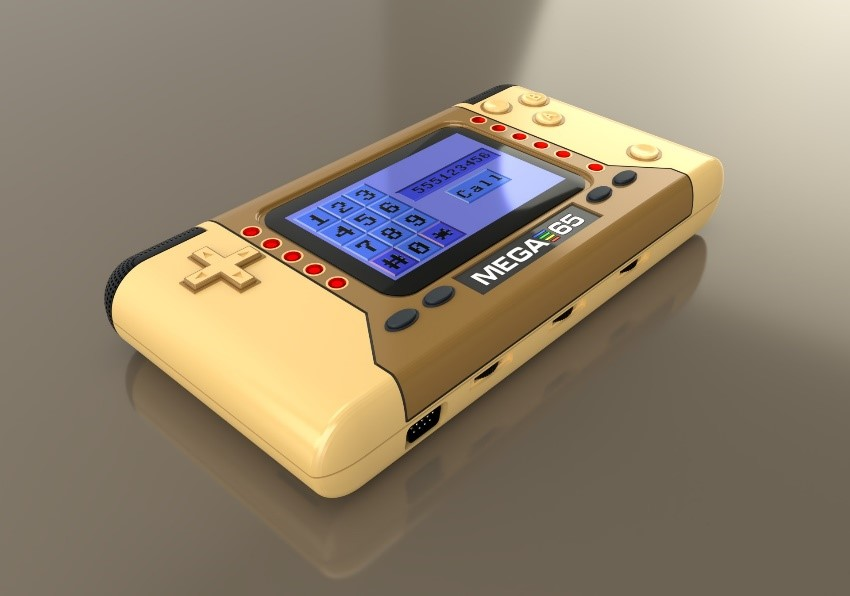
\includegraphics[width=\linewidth]{render.jpg}
	\caption{MEGAPhone Prototype Render}
	\label{fig:render}
\end{figure}

The secure device will have the capability to be able to disconnect from the world by having a mechanical switch to power its modem on and off, as well as having an advanced encryption system and multiple SIM card slots.
The phone will be designed for security over functionality, in contrast to many modern smartphones.
All design choices including the routing stage of the PCB will be completed with security in mind, with an FPGA board being used as the CPU.

One of the major challenges in making the device fully secure, is ensuring that the modem can be turned on and off, when desired without directly affecting the state of the other components. 
	Research is needed in this topic due to the increasing risks in computer security, and the lack of secure mobile devices, considering the age in which we live in where everyone’s personal details are linked to their smartphones.

%----------------------------------------------------------------------------------------
%	SECTION 7
%----------------------------------------------------------------------------------------

\section{Design Software}
\label{chap2sec8}

Altium Designer is a software-based schematic and PCB design program.
The software has the ability to create complex designs, of any nature – accurately.
There are also a number of debugging tools within the program. 
The project will use Altium Designer as the primary design platform, for both the schematic and PCB designs.
This will ensure both fluidity and efficiency, during the design phase. 
Compared to other PCB design programs Altium Designer provides a higher level of functionality and usability.
Other programs including KiCad and Altium Circuit Maker provide schematic and PCB design options but with less functionalities and fluidity within the programs. 
